% ----------------------------------------------------------------------------------
% A LIST OF EXPERIMENTS TO DO 
% ----------------------------------------------------------------------------------
\section{Case Study 1}
%\chapter{Case Study 1}
\label{sect:cs1_study}
This investigation involves running a series of one-night simulations under different environmental assumptions to see the effect of varying the value of the SHM weights $w_{trans}$ relative to the priority weight $w_p$.
The rational behind this investigation is to provide some initial insight into the usefulness of the various SQMs and to provide a shakedown test of the simulation framework on real data. By selecting 2 seperate but similar nights it should be possible to get a preliminary idea on the range of likely values fand variation of SQMs.


 The set of \emph{remaining} objective function weights ${W_x}$ excluding $w_{trans}$ and $w_p$ are kept constant at zero level throughout the range of test values to avoid any additional biasing. The SQMs used to evaluate the quality of the resulting schedules are $Q_{OA}$ - the optimal airmass metric, $Q_{PX}$ - the execution time weighted priority metric, $Q_{RN}$ - urgency metric, $Q_{TD}$ - demand metric, $Q_{PX \cdot OA}$ - priority weighted optimal airmass and $Q_X$ the total execution time as a fraction of available night. 

Two nights were considered. Both were similar in terms of amount of dark moon time though the actual night lengths were significantly different. Night 1, 13th-14th October 2007 has xxx hours of lunar dark time out of xxx hours night of which xxx hours are astronomicaly dark. Night 2, 7th-8th November 2007 has xxx hours of lunar dark time out of xxx hours night of which xxx hours are astronomicaly dark.


\begin{table}
\begin{center}
\caption{Case study night characteristics}
\begin{tabular}{lll}
\toprule
\multicolumn{2}{c}{Case study night characteristics} \\
\midrule
Item & Night 1 & Night 2 \\
\midrule
Date                & 14-15 Oct 2007 & 7-8 Nov 2007\\
Sunset              & 18:40          & 18:20\\
Sunrise             & 07:08          & 07:23\\
Start Astro night   & 19:58          & 19:40\\
End Astro night     & 05:50          & 06:03\\
Moonset             & 10:01          & 16:47\\
Moonrise            & 20:27          & 06:05\\
\midrule
Length of night     & 12:28          & 13:03\\
Length astro night  & 9:52           & 10:23\\
Length astro moon dark    & 7:23     & 10:03\\
Lunar dark fraction & 75\%           & 96.7\%\\
\bottomrule
\end{tabular}
\end{center}
\end{table}

A series of simulations were performed to determine the range of contention statistics for the 2 study nights. Figures \ref{fig:cont4_ensemble} and \ref{fig:cont6_ensemble} show ensemble results from a large number of simulations for the 2 nights.d \ref{fig:bsa1_ex}.

\begin{figure}[h]
 \begin{center}
  \subfigure[Contention profile $C_c$ ensemble for night 2.] {
    \label{fig:cont4_ensemble}
    \includegraphics[scale=0.25, angle=-90]{figures/cont4_ensemble.eps}
  }
  \subfigure[Contention profile $C_c$ ensemble for night 1.] {
    \label{fig:cont6_ensemble}
    \includegraphics[scale=0.25, angle=-90]{figures/cont6_ensemble.eps}
  }
\caption{Contention profile ensembles for case study nights 1 and 2} 
 \end{center}
\end{figure}

A comparison for several runs using fixed execution models and various environmental models are displayed in figures \ref{fig:bsa0_pr} and \ref{fig:bsa0_pr} (Wrong labels !)

\begin{figure}[h]
 \begin{center}
 \subfigure[Variation of contention profile $C_c$ under $E_{FP}$ night 1.] {
   \label{fig:bsa0_pr}
   \includegraphics[scale=0.25, angle=-90]{figures/bsa_pr_cont.eps}
  }
 \subfigure[Variation of contention profile $C_c$ under $E_{FX}$ night 1.] {
   \label{fig:bsa1_ex}
   \includegraphics[scale=0.25, angle=-90]{figures/bsa_ex_cont.eps}
  } 
  
  \subfigure[Variation of contention profile $C_c$ under $E_{RA}$ night 1.] {
   \label{fig:bsa2_rnd}
   \includegraphics[scale=0.25, angle=-90]{figures/bsa_rnd1_cont.eps}
  }
  \subfigure[Variation of contention profile $C_c$ under $E_{RA}$ night 1.] {
   \label{fig:bsa2_rnd}
   \includegraphics[scale=0.25, angle=-90]{figures/bsa_rnd2_cont.eps}
  } 

   \subfigure[Variation of contention profile $C_c$ under mixed environment for night 1.] {
   \label{fig:bsa2_rnd}
   \includegraphics[scale=0.25, angle=-90]{figures/bsa_combine_cont.eps}
  }
  \caption{Effects of environment model on contention profile for night 1}
 \end{center}
\end{figure}

\begin{figure}[h]
 \begin{center}
 \subfigure[Variation of contention profile $C_c$ under $E_{FP}$ night 2.] {
   \label{fig:bsa0_pr}
   \includegraphics[scale=0.25, angle=-90]{figures/bsb_pr_cont.eps}
  }
 \subfigure[Variation of contention profile $C_c$ under $E_{FX}$ night 2.] {
   \label{fig:bsa1_ex}
   \includegraphics[scale=0.25, angle=-90]{figures/bsb_ex_cont.eps}
  }
  
  \subfigure[Variation of contention profile $C_c$ under $E_{RA}$ night 2.] {
   \label{fig:bsa2_rnd}
   \includegraphics[scale=0.25, angle=-90]{figures/bsb_rnd1_cont.eps}
  }
  \subfigure[Variation of contention profile $C_c$ under $E_{RA}$ night 2.] {
   \label{fig:bsa2_rnd}
   \includegraphics[scale=0.25, angle=-90]{figures/bsb_rnd2_cont.eps}
  } 

   \subfigure[Variation of contention profile $C_c$ under mixed environment for night 2.] {
   \label{fig:bsa2_rnd}
   \includegraphics[scale=0.25, angle=-90]{figures/bsb_combine_cont.eps}
  }
 \caption{Effects of environment model on contention profile for night 2}
  
 \end{center}
\end{figure}


For both nights simulations were run using a basic rank scoring selection mechanism $\mathcal{S}_{BEST}$ which selects the highest scoring group from the set of candidate metrics. In addition a second simulation was performed using a random selection model $\mathcal{S}_{Random}$ in which all candidates have equal chance of selection irrespective of their relative scores. This was to provide an indication of how well the normal selection and scoring mechanisms perform against a baseline.

The following models were fixed in all cases:-
\begin{itemize}
 \item Charge Accounting Model $\mathcal{C}$ is described in \ref{tab:cam_param}.
 \item Scoring model $\mathcal{S}$ was setup initially with no weighting parameters as these are to be varied during the experment.
 \item Execution timing and feasibility model $X$ is described in \ref{tab:etm_param}.
 \item Stochastic execution mode $\mathcal{\zeta}$ is described in \ref{tab:sex_param}.
\end{itemize}

\clearpage
\begin{landscape}
\begin{table}
\begin{center}
\caption{Fixed model parameters for all simulations}
\centering
\subtable[Charge accounting model parameters. These are used to work out the accounting debit on completion of a group execution]{
\label{tab:cam_param}
\begin{tabular}{ll}
\toprule
\multicolumn{2}{c}{Charge Accounting Model} \\
\midrule
Accounting parameter & Value(sec) \\
\midrule
Offset & 10\\
Slewing rotation & 60 \\
Instrument configuration & 5 \\
Instrument readout & 12\\
\bottomrule
\end{tabular}
}
\subtable[Execution timing and feasibility  model parameters. These are used to determine whether a group can execute at a given time under specified environmental conditions and with given execution history and to \emph{estimate} how long it is likely to take]{
\label{tab:etm_param}
\begin{tabular}{lll}
\toprule
\multicolumn{3}{c}{Execution Feasibility and Timing Model} \\
\midrule
Execution model parameter & Value & Units \\
\midrule
Dome horizon & 20 & $^{\circ}$\\
Dome zenith limit & 89 & $^{\circ}$ \\
Solar night elevation & -18 & $^{\circ}$ \\
Dark twilight elevation & -12.0 & $^{\circ}$\\
Bright twilight elevation & -6.0  & $^{\circ}$\\
Fixed group pre-start buffer & 200 & sec\\
Fixed group post-start lapse & 900 & sec\\
Max execution time & 7200 & sec\\
Offset & 10 & sec\\
Slewing rotation & 60 & sec \\
Instrument configuration & 6 &sec \\
Instrument readout & 12 & sec\\
\bottomrule
\end{tabular}
}
\subtable[Lost the description]{
\label{tab:sex_param}
\begin{tabular}{lll}
\toprule
\multicolumn{3}{c}{Stochastic Execution Timing  Model} \\
\midrule
Execution timing parameter & Minimum value (sec) & Maximum value (sec) \\
\midrule
Offset & 5 & 12\\
Slewing rotation & 30 & 120 \\
Instrument configuration & 6 & 12 \\
Instrument readout & 8 & 13\\
\bottomrule
\end{tabular}     
}
\end{center}
\end{table}
\end{landscape}

Results of the random selection models were as follows:-

\clearpage
% RS4
\begin{table}
\begin{center}
\begin{tabular}{lllllll}
\toprule
\multicolumn{7}{c}{Results for Random slection model $\zeta_{random}$} \\
\midrule
Metric & $Q_{OA}$ & $Q_{PX}$ & $Q_{TD}$ & $Q_{X}$ & $Q_{RN}$ & $Q_{PX \cdot OA}$ \\
\midrule
{\bf Average} & 0.835  & 1.332  & 2.957  & 0.907  & 23.976 & 1.086\\
{\bf Minimum} & 0.775  & 0.921  & 1.417  & 0.881  & 15.331 & 0.765\\
{\bf Maximum} & 0.887  & 1.698  & 5.000  & 0.932  & 33.225 & 1.417\\
{\bf SDev}    & 0.0225 & 0.1357 & 0.8021 & 0.0081 & 3.6253 & 0.1258\\
\bottomrule
\end{tabular}
\end{center}
\caption{Results for Night 1 under $E_{FP}$}
\end{table}

% RS5
\begin{table}
\begin{center}
\begin{tabular}{lllllll}
\toprule
\multicolumn{7}{c}{Results for Random slection model $\zeta_{random}$} \\
\midrule
Metric & $Q_{OA}$ & $Q_{PX}$ & $Q_{TD}$ & $Q_{X}$ & $Q_{RN}$ & $Q_{PX \cdot OA}$ \\
\midrule
{\bf Average} & 0.817  & 1.217  & 2.851  & 0.929  & 21.339 & 0.999\\
{\bf Minimum} & 0.771  & 0.817  & 1.096  & 0.908  & 10.410 & 0.643\\
{\bf Maximum} & 0.875  & 1.510  & 4.842  & 0.956  & 30.924 & 1.346\\
{\bf SDev}    & 0.023  & 0.1268 & 0.7203 & 0.0079 & 3.5596 & 0.1179\\
\bottomrule
\end{tabular}
\end{center}
\caption{Results for Night 1 under $E_{FX}$}
\end{table}

% RS6
\begin{table}
\begin{center}
\begin{tabular}{lllllll}
\toprule
\multicolumn{7}{c}{Results for Random slection model $\zeta_{random}$} \\
\midrule
Metric & $Q_{OA}$ & $Q_{PX}$ & $Q_{TD}$ & $Q_{X}$ & $Q_{RN}$ & $Q_{PX \cdot OA}$ \\
\midrule
{\bf Average} & 0.826  & 0.966  & 3.580  & 0.860  & 23.605 & 0.797\\
{\bf Minimum} & 0.782  & 0.644  & 1.916  & 0.834  & 16.081 & 0.548\\
{\bf Maximum} & 0.866  & 1.233  & 5.236  & 0.875  & 30.205 & 1.065\\
{\bf SDev}    & 0.0165 & 0.1174 & 0.6754 & 0.0063 & 2.6545 & 0.1013\\
\bottomrule
\end{tabular}
\end{center}
\caption{Results for Night 2 under $E_{FX}$}
\end{table}

% RS7
\begin{table}
\begin{center}
\begin{tabular}{lllllll}
\toprule
\multicolumn{7}{c}{Results for Random slection model $\zeta_{random}$} \\
\midrule
Metric & $Q_{OA}$ & $Q_{PX}$ & $Q_{TD}$ & $Q_{X}$ & $Q_{RN}$ & $Q_{PX \cdot OA}$ \\
\midrule
{\bf Average} & 0.811  & 0.812  & 3.930  & 0.900  & 28.765 & 0.669\\
{\bf Minimum} & 0.745  & 0.575  & 2.079  & 0.885  & 20.535 & 0.439\\
{\bf Maximum} & 0.864  & 1.118  & 6.264  & 0.908  & 40.172 & 0.908\\
{\bf SDev}    & 0.0221 & 0.1123 & 0.8007 & 0.0038 & 3.746 & 0.1020\\
\bottomrule
\end{tabular}
\end{center}
\caption{Results for Night 2 under $E_{FX}$}
\end{table}

First results revealed a surprisingly minor effect of varying $w_{trans}$ especially at values of $w_{trans}$ from 0 to 50\% where the plot is particularly flat. The plot then rises rapidly at some cut-in point - further investigation is suggested to see if the cut-in point depends on environment and load factors. In addition the non-linear domain sampling suggested the need for a different regime of domain sampling. 


\clearpage
\begin{figure}[h]
 \begin{center}
  \subfigure[Effect of varying $w_{trans}$ relative to $w_{p}$ on $Q_{PX}$ schedule quality metric]{
    \label{fig:cs1_dw1_px}
    \includegraphics[scale=0.25, angle=-90]{figures/cs1_dw1_px.eps}
  }
  \subfigure[Effect of varying $w_{trans}$ relative to $w_{p}$ on $Q_{OA}$ schedule quality metric]{
    \label{fig:cs1_dw1_oa}
    \includegraphics[scale=0.25, angle=-90]{figures/cs1_dw1_oa.eps}
  }
  \subfigure[Effect of varying $w_{trans}$ relative to $w_{p}$ on $Q_{OA}$ schedule quality metric for Flexible groups]{
    \label{fig:cs1_dw1_foa}
    \includegraphics[scale=0.25, angle=-90]{figures/cs1_dw1_foa.eps}
  }
  \subfigure[Effect of varying $w_{trans}$ relative to $w_{p}$ on $Q_{PX}$ schedule quality metric for Flexible groups]{
    \label{fig:cs1_dw1_fpx}
    \includegraphics[scale=0.25, angle=-90]{figures/cs1_dw1_fpx.eps}
  }
  \subfigure[Effect of varying $w_{trans}$ relative to $w_{p}$ on $Q_{TD}$ schedule quality metric]{
    \label{fig:cs1_dw1_td}
    \includegraphics[scale=0.25, angle=-90]{figures/cs1_dw1_td.eps}
  }
  \subfigure[Effect of varying $w_{trans}$ relative to $w_{p}$ on $Q_{RN}$ schedule quality metric]{
    \label{fig:cs1_dw1_rn}
    \includegraphics[scale=0.25, angle=-90]{figures/cs1_dw1_rn.eps}
  }
\caption{Results for night 2 (7-8 November 2007) for environment model $E_{FP}$} 
 \end{center}
\end{figure}


\clearpage
\begin{figure}[h]
 \begin{center}
  \subfigure[Effect of varying $w_{trans}$ relative to $w_{p}$ on $Q_{PX}$ schedule quality metric]{
    \label{fig:cs1_dw1_px}
    \includegraphics[scale=0.25, angle=-90]{figures/cs1_dw2_px.eps}
  }
  \subfigure[Effect of varying $w_{trans}$ relative to $w_{p}$ on $Q_{OA}$ schedule quality metric]{
    \label{fig:cs1_dw1_oa}
    \includegraphics[scale=0.25, angle=-90]{figures/cs1_dw2_oa.eps}
  }
  \subfigure[Effect of varying $w_{trans}$ relative to $w_{p}$ on $Q_{OA}$ schedule quality metric for Flexible groups]{
    \label{fig:cs1_dw1_foa}
    \includegraphics[scale=0.25, angle=-90]{figures/cs1_dw2_foa.eps}
  }
  \subfigure[Effect of varying $w_{trans}$ relative to $w_{p}$ on $Q_{PX}$ schedule quality metric for Flexible groups]{
    \label{fig:cs1_dw1_fpx}
    \includegraphics[scale=0.25, angle=-90]{figures/cs1_dw2_fpx.eps}
  }
  \subfigure[Effect of varying $w_{trans}$ relative to $w_{p}$ on $Q_{TD}$ schedule quality metric]{
    \label{fig:cs1_dw1_td}
    \includegraphics[scale=0.25, angle=-90]{figures/cs1_dw2_td.eps}
  }
  \subfigure[Effect of varying $w_{trans}$ relative to $w_{p}$ on $Q_{RN}$ schedule quality metric]{
    \label{fig:cs1_dw1_rn}
    \includegraphics[scale=0.25, angle=-90]{figures/cs1_dw2_rn.eps}
  }
\caption{Results for night 2 (7-8 November 2007) for environment model $E_{FX}$} 
 \end{center}
\end{figure}
 
\clearpage
% comparison graphs
\begin{figure}[h]
\begin{center}
  \subfigure[Comparison of effect of environment model ($E_{FP}$, $E_{FX}$) on $Q_{OA}$ for variable $w_{trans}$.]{
   \includegraphics[scale=0.25, angle=-90]{figures/cs1_dw1a2_oa.eps}
   \label{fig:cs1_dw1a2_oa}
  }
  \subfigure[Comparison of effect of environment model ($E_{FP}$, $E_{FX}$) on $Q_{PX}$ for variable $w_{trans}$.] {
    \includegraphics[scale=0.25, angle=-90]{figures/cs1_dw1a2_px.eps}
    \label{fig:cs1_dw1a2_px}
  }
  \subfigure[Comparison of effect of environment model ($E_{FP}$, $E_{FX}$) on $Q_{RN}$ for variable $w_{trans}$.] {
    \includegraphics[scale=0.25, angle=-90]{figures/cs1_dw1a2_rn.eps}
     \label{fig:cs1_dw1a2_rn}
  }
  \subfigure[Comparison of effect of environment model ($E_{FP}$, $E_{FX}$) on $Q_{TD}$ for variable $w_{trans}$.] {
    \includegraphics[scale=0.25, angle=-90]{figures/cs1_dw1a2_td.eps}
    \label{fig:cs1_dw1a2_td}
  }
  \subfigure[Comparison of dependancy of $Q_{OA}$ on $w_{trans}$ for all groups and flexible groups under environment model $E_{FP}$.]{
    \includegraphics[scale=0.25, angle=-90]{figures/cs1_dw1_oa_c.eps}
    \label{fig:cs1_dw1_oa_c}
  }
  \subfigure[Comparison of dependancy of $Q_{PX}$ on $w_{trans}$ for all groups and flexible groups under environment model $E_{FP}$.]{
    \includegraphics[scale=0.25, angle=-90]{figures/cs1_dw1_px_c.eps}
    \label{fig:cs1_dw1_px_c}
  }
 \caption{Results for night 2 (7-8 November 2007) for variable environment models.}
\end{center}
\end{figure}

